
\documentclass[12pt,article]{memoir}

\usepackage{fancyhdr}
\usepackage{graphicx}
\usepackage{fontspec}
\setmainfont{Calibri}
\usepackage{tikz}
\usetikzlibrary{calc}
\usepackage{xcolor}
\usepackage{xpatch}
\usepackage{hyperref}

\usepackage{fancyhdr}
\usepackage{graphicx}
\usepackage{fontspec}
\setmainfont{Calibri}
\usepackage{tikz}
\usetikzlibrary{calc}
\usepackage{xcolor}
\usepackage{xpatch}
\usepackage{hyperref}
\usepackage{tabu}
\usepackage{float}
\usepackage[autostyle, english = american]{csquotes}


\usepackage[yyyymmdd]{datetime} % change date format to yyyy/mm/dd to fit ISO8601

\renewcommand{\familydefault}{\sfdefault} % set font
\renewcommand{\dateseparator}{--} % change date-seperators to - to fit ISO8601

\renewcommand\contentsname{Table of Contents}

\chapterstyle{section}
\renewcommand*{\chapnumfont}{\normalfont\HUGE\bfseries\sffamily}
\renewcommand*{\chaptitlefont}{\normalfont\HUGE\bfseries\sffamily}

\makeatletter 
% define macro for itemcode
\newcommand\itemcode[1]{\renewcommand\@itemcode{#1}}
\newcommand\@itemcode{}

% define macro for rev number
\newcommand\revnumber[1]{\renewcommand\@revnumber{#1}}
\newcommand\@revnumber{}
\makeatother

\definecolor{orbitOrange}{RGB}{250,62,0} % the ORBiT orange

\setlrmarginsandblock{2.5cm}{2.5cm}{*}
\setulmarginsandblock{2.5cm}{*}{1}
\checkandfixthelayout 

\setlength{\beforechapskip}{0cm} % reduce chapter spacing

\hypersetup{
    colorlinks,
    citecolor=black,
    filecolor=black,
    linkcolor=black,
    urlcolor=black
}

%**********************************************************************
%Document titles etc. defined here: (replace [] as well)
\title{ORBiT Avionics System II Architecture}
\author{Jinzhi Cai}
\itemcode{Sys-Arch}
\revnumber{A02}
\date{\today}
%end of document titles etc.
%**********************************************************************

\makeatletter
\let\runtitle\@title
\let\runitemcode\@itemcode
\makeatother

% set header style
\pagestyle{fancy}
{
	\fancyheadoffset{0cm}

	\lhead{\runtitle \ - \runitemcode}
	\rhead{Page: \thepage }
	%\chead{\leftmark} % section name
}

\newcommand{\OrbitBackground}{% For a logo drawn with TikZ
\begin{tikzpicture}[remember picture,overlay] % draw background
	\coordinate (bl) at (current page.south west);
	\coordinate (r) at (current page.east);
    \coordinate (A) at ($(bl)+(0,3cm)$);
    \coordinate (B) at ($(r)+(0,-2cm)$);
    \coordinate (C) at (current page.south east);
    \coordinate (ctrlNode) at ($(current page.south) + (0cm,1cm)$);
    \coordinate (ctrlNode2) at ($(current page.south east) + (-1cm,1cm)$);
    \fill[orbitOrange, fill opacity=0.2]
    (A) .. controls (ctrlNode) and (ctrlNode2) .. (B) -- (C) -- (bl);
    \node [white] at ($(C) + (-3cm,1cm)$) {2015-\the\year \ ORBiT@SU};
\end{tikzpicture}
}

\cfoot{\OrbitBackground}

\begin{document}

\begin{tikzpicture}[remember picture,overlay] % draw background
	\coordinate (bl) at (current page.south west);
	\coordinate (r) at (current page.east);
    \coordinate (A) at ($(bl)+(0,3cm)$);
    \coordinate (B) at ($(r)+(0,-2cm)$);
    \coordinate (C) at (current page.south east);
    \coordinate (ctrlNode) at ($(current page.south) + (0cm,1cm)$);
    \coordinate (ctrlNode2) at ($(current page.south east) + (-1cm,1cm)$);
    \fill[orbitOrange]
    (A) .. controls (ctrlNode) and (ctrlNode2) .. (B) -- (C) -- (bl);
    \node [white] at ($(C) + (-3cm,1cm)$) {2015-\the\year \ ORBiT@SU};
\end{tikzpicture}

\makeatletter
	
\includegraphics[width=\textwidth]{../logo.jpg}\\[4ex]
	\begin{center}
	{\fontsize{50}{60}\selectfont \bfseries  \@title }\\[2ex] 
	{\LARGE  \@itemcode}\\
	\end{center}
	\begin{flushright}
	\vspace*{\fill}
	{\LARGE Rev: \@revnumber}\\[2ex]
	{\large \@author}\\[2ex]
	{\large \@date}\\[20ex]
	\end{flushright}
\makeatother
\thispagestyle{empty}
\newpage

\tableofcontents*
\thispagestyle{fancy}
\newpage

%**********************************************************************
% Everything after this is the main document. Edit below this line,
\chapter{General Software System Architecture}
The software system for OA-II can be divided to three layers: data link layer, Transport layer, and application layer.
\begin{figure}[htp]
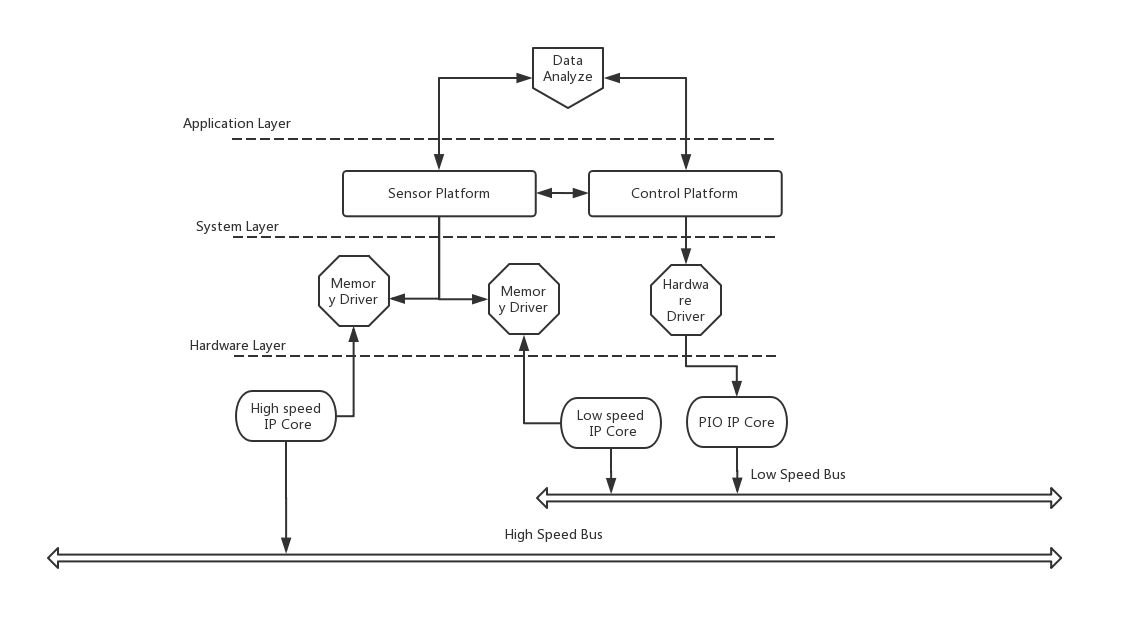
\includegraphics[width=\textwidth]{softarch.png}
\caption{Software Architecture}	
\end{figure}
\section{Data Link Layer}
The data link layer directly interacts with hardware memory. It include drivers for all hardware buses. It also includes programs which execute direction on the CPU.
\section{Transport Layer}
The transport layer connects the data link and application layers. It receives data from different data link layer sources and packetizes it. It will feed all the packetized data to relevant application program. It provides critical control before and during the flight. Finally, the transport layer records all data to onboard storage.
\section{Application Layer}
The application layer is used to process data provided by the transport layer, as well as to provide information that will be sent back to OA-II BAS.

\newpage

\chapter{General Hardware System Architecture}
\section{Payload Catalog}
\subsection{Critical Payload}
The critical payload controls basic launch and recovery operations. It will attach directly to the Compute Module (CM). Any failure of the critical payload will result in a launch abort. The critical payload contains:
\begin{itemize}
\item Power management
\item GPS receiver
\item Low speed IMU
\item Storage media
\item Radio system
\end{itemize}

\subsection{High Speed Payload} - The high speed payload contains non-critical devices, in particular sensors. This payload is primarily for research purposes. These devices will be located in the Telemetry Module (TM), and include:
\begin{itemize}
\item Static and dynamic air pressure sensors
\item High speed IMU
\item Cameras
\item Temperature sensors
\item Pressure sensors
\end{itemize}

\subsection{Low Speed Payload} - The low speed payload contains non-critical devices which are significant EMI sources. The low speed payload must be fully galvanically isolated from the rest of the system. This includes:
\begin{itemize}
\item Actuators
\item Pyrotechnics
\end{itemize}
\begin{figure}[htp]
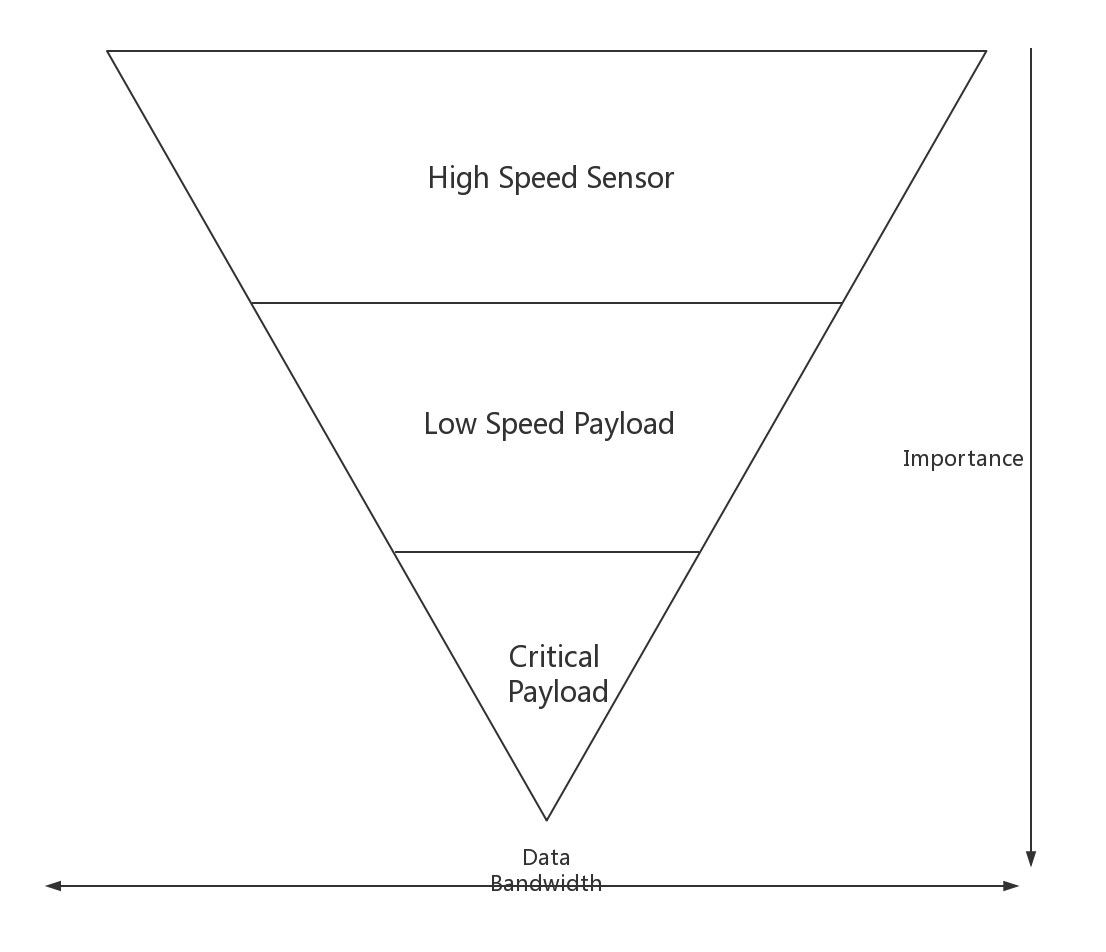
\includegraphics[width=\textwidth]{payloadCata.png}
 \caption{Payload Diagram}	
\end{figure}
%*************************************************************************************
%*************************************************************************************
%*************************************************************************************

\newpage

\chapter{Vehicle Electronics (VEH) System Architecture}
\section{Description}
The OA-II VEH is a compact, modular system which is tightly integrated with the flight vehicle.
\section{Payload Frame (PF)}
The Payload Frame (PF) contains interchangeable modules and provides a high speed bus controller and power supply. The PF should be a four layer board.
\section{Payload Modules (PM)}
Payload Modules are specialized circuits which slot into the Payload Frame. They can be divided into three primary types: Computing Modules (CM), Telemetry Modules (TM), and Power and Actuator Module (PAM).
\subsection{Compute Module (CM)}
The Compute Module (CM) has several purposes. It controls other modules and monitors the vehicle status. It collects data from Telemetry Modules, and contains long-term storage for collected data. 
\subsection{Telemetry Module (TM)}
The Telemetry Module (TM) is an interface to both sensors and radios. The TM connects to both low and high speed sensors. The TM also FIFO buffers for high speed sensors.
%*****************************************************************************
\subsection{Power and Actuator Module (PAM)}%Use for landing?
The Power and Actuator Module (PAM) is providing power and operating any mechanical component. It manage the main power source of the vehicle and allow CM to control high power electronic. The PAM also offer limited control for safety cutoff in case CM lost connection or power.
%\subsection{Adaptable Rockets}
%\section{PCB Layout Description}%\section{PCB Layout and Manufacture Description}
%\subsection{PCB Layout}
%\subsection{PCB Manufacture Requirement}
%***************************************************************************
%**********************************************************************
%**********************************************************************

\newpage

\chapter{Base Station Electronics (BAS) System Architecture}
\section{General Description}
The OA-II BAS is a modular launch pad and flight control center. It performs three major functions: launch control operations, live data analysis and display, and vehicle status indication.
\section{Launch Control}
The Launch Control Module monitors and controls the vehicle before, during, and after flight. This includes ignition and oxidizer control, parameter tuning, and launch abort functionality.
\section{Live Data}
The Live Data Module shows vehicle information during flight. This includes a 3D map of the flight path, propulsion system temperatures and pressures, and IMU data.
\section{Vehicle Status}
The Vehicle Status Module performs basic analysis on the live telemetry data. This includes displaying a Range Safe/Range Live indication, vehicle orientation from sensor fusion, flight profile stages, and error monitoring.
%***************************************************************************
%**********************************************************************s

\newpage

\chapter{Backplane System (BPS) Architecture}
\section{General Description}
The OA-II BPS is the main bus system for all the OA-II relative component. It will provide up to 500MB/s band width. In the same time, it also provide low data lane for smaller component and low power, sample application. It also provide 24V power for all the module that attach with it.
\begin{figure}[h]
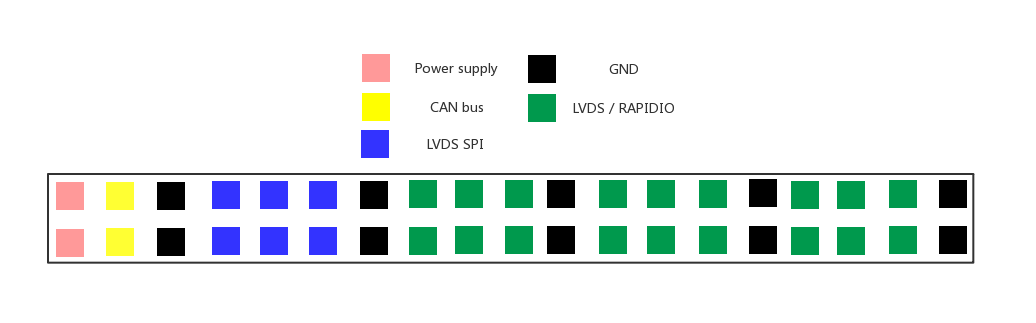
\includegraphics[width=\textwidth]{BPS_Pin.png}
 \caption{Example Pin Out}	
\end{figure}
%\section{System Description}
%\section{Backplane Connection Protocal}
%\subsection{Connection Protocal}
%\subsection{Pin Diagram}
%***************************************************************************

\newpage

\chapter{Wireless System (WLS) Architecture}
\section{General Description}
The ORBiT Avionics II Wireless System (OA-II WLS) is use to connect vehicle and base station. It is important part of OA-II STAM and OA-II "Demonstrator". The OA-II WLS provide two type of communication between the vehicle and base station, the high speed mode and low power mode.
\section{High Speed Wireless Connection Protocal}
The OA-II HSWLS is use mainly during the fly and allow to provide high speed communication to the base station. It will download live vehicle status and video stream to the base station.
\section{Low Power Wireless Connection Protocal}
The OA-II LPWLS is mainly use for landing and component recovery. It provide location tracing and boardcast system and also allow radio locating in range.

\chapter{Revision History}
\begin{table}[H]
	\centering
	\begin{tabu}{r || c | c | c }
		Rev\# & Editor & Delta & Date\\ \hline
		A01 & Jinzhi Cai & Initialize  & 2019-6-27\\ \hline
		A02 & .... & ....  & 2019-6-28
	\end{tabu}
	\caption{Summary of Revision History}
	\label{tab:edatools}
\end{table}
%\section{System Description}
%\section{}
%\section{}
%end of document
%**********************************************************************
\end{document}

%\begin{table}[H]
%	\centering
%	\begin{tabu}{r || c | c  }
%		Rocket Series & Part Number & Date\\ \hline
%		 ?& ?& ?\\
%		 & & \\
%		 & & \\ 
%		 & & \\
%	\end{tabu}
%	\caption{Adaptable Rockets}
	%\label{tab:edatools}
%\end{table}
%
